\documentclass[tikz,border=4pt]{standalone}
\usepackage[T1]{fontenc}
\usepackage{lmodern}
\usetikzlibrary{arrows.meta,positioning,fit,backgrounds,calc,shapes.geometric,decorations.pathreplacing}
\begin{document}
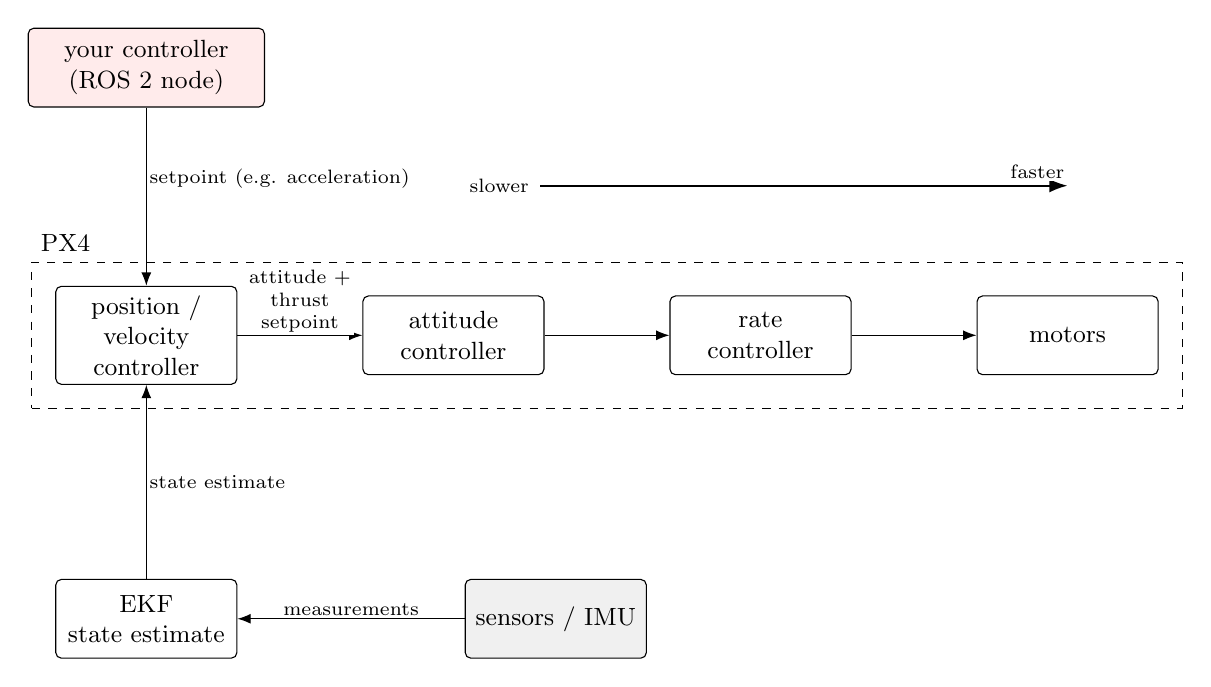
\begin{tikzpicture}[
  blk/.style={draw,rounded corners=2pt,minimum height=10mm,minimum width=23mm,align=center,font=\small,fill=white},
  ros/.style={blk,fill=red!8},
  ext/.style={blk,fill=gray!12},
  lab/.style={font=\scriptsize,fill=white,inner sep=1pt,align=center},
  >={Latex}]
\node[ros,minimum width=30mm] (ctl) at (0,0) {your controller\\(ROS 2 node)};
\node[blk] (pv) at (0,-3.4) {position /\\velocity\\controller};
\node[blk] (att) at (3.9,-3.4) {attitude\\controller};
\node[blk] (rate) at (7.8,-3.4) {rate\\controller};
\node[blk] (mot) at (11.7,-3.4) {motors};
\begin{scope}[on background layer]
\node[draw,dashed,inner sep=3mm,fit=(pv)(att)(rate)(mot)] (px) {};
\end{scope}
\node[font=\small,anchor=south west] at (px.north west) {PX4};
\node[blk] (ekf) at (0,-7) {EKF\\state estimate};
\node[ext] (sen) at (5.2,-7) {sensors / IMU};
\draw[->] (ctl) -- node[lab,right,pos=0.4]{setpoint (e.g. acceleration)} (pv);
\draw[->] (pv) -- node[lab,above]{attitude +\\thrust\\setpoint} (att);
\draw[->] (att) -- (rate);
\draw[->] (rate) -- (mot);
\draw[->] (sen) -- node[lab,above]{measurements} (ekf);
\draw[->] (ekf.north) -- node[lab,right]{state estimate} (pv.south);
\draw[->,thick] (5,-1.5) -- (11.7,-1.5);
\node[lab,anchor=east] at (4.9,-1.5) {slower};
\node[lab,anchor=south east] at (11.7,-1.45) {faster};
\end{tikzpicture}
\end{document}
